\documentclass[sigconf, nonacm, language=english, language=portuguese, natbib=false]{acmart}

%% ---------------------------------------------------------------------------
%% Bibliografia: o acmart com natbib=false exige biblatex com o estilo
%% acmnumeric. (A versão anterior carregava o biblatex DUAS vezes, com estilos
%% diferentes, o que gerava "Option clash for package biblatex".)
%% No Overleaf: Menu > Settings > Compiler = pdfLaTeX (o biber roda sozinho).
%% ---------------------------------------------------------------------------
\RequirePackage[datamodel=acmdatamodel, style=acmnumeric]{biblatex}
\addbibresource{referencias.bib}

\usepackage{csquotes}
\usepackage{tikz}
\usetikzlibrary{positioning, arrows.meta}

%% Marca tudo que ainda depende dos experimentos. Para achar o que falta:
%% Ctrl+F "\pendente". Antes de entregar, nenhuma marcação vermelha deve sobrar.
\newcommand{\pendente}[1]{\textcolor{red}{\textbf{[#1]}}}

\AtBeginDocument{\providecommand\BibTeX{{Bib\TeX}}}

%% Artigo de especialização (não publicado pela ACM): a opção "nonacm" remove
%% cabeçalho de conferência, caixa de copyright e "ACM Reference Format".
\setcopyright{none}

\begin{document}

\title{Obtenção de dados de rastreamento ocular com webcam utilizando Inteligência Artificial para avaliação da experiência do usuário}

\author{Bruno M. Ribas}
\email{brunoribas68@gmail.com}
\affiliation{%
  \institution{Setor de Educação Profissional e Tecnológica, Universidade Federal do Paraná}
  \city{Curitiba}
  \state{Paraná}
  \country{Brasil}
}

\author{Jaime Wojciechowski}
\email{jaimewo@ufpr.br}
\affiliation{%
  \institution{Setor de Educação Profissional e Tecnológica, Universidade Federal do Paraná}
  \city{Curitiba}
  \state{Paraná}
  \country{Brasil}
}

\begin{abstract}
O rastreamento ocular permite observar para onde os usuários olham ao interagir com um produto digital e é uma fonte valiosa de dados para avaliar a experiência do usuário (UX). Contudo, rastreadores dedicados são caros e exigem laboratório, o que limita seu uso. Este trabalho, apresentado como conclusão da Especialização em Inteligência Artificial Aplicada, desenvolve e avalia um protótipo de rastreamento ocular que utiliza apenas uma webcam comum. O sistema detecta o rosto e a íris com uma rede neural convolucional (MediaPipe Face Mesh), aprende por regressão regularizada o mapeamento entre a posição da íris e a tela a partir de uma calibração de nove pontos, suaviza o sinal com o filtro One Euro e segmenta fixações com o algoritmo I-DT, gerando mapas de calor, trajetórias do olhar e métricas por área de interesse. Em um experimento com \pendente{N} participantes, o sistema obteve acurácia média de \pendente{X}$^\circ$ de ângulo visual, precisão de \pendente{Y}$^\circ$ e perda de dados de \pendente{Z}\%. \pendente{Uma frase de conclusão: por exemplo, a precisão obtida é suficiente para identificar quais regiões de uma página atraem a atenção, mas não para análises em nível de palavra.} O código é aberto e reprodutível.
\end{abstract}

\begin{translatedabstract}{english}
Eye tracking reveals where users look while interacting with a digital product and is a valuable data source for user experience (UX) evaluation. However, dedicated eye trackers are expensive and require a laboratory, which limits their adoption. This work, the final paper of the Specialization in Applied Artificial Intelligence, develops and evaluates an eye-tracking prototype that relies solely on a commodity webcam. The system detects the face and iris with a convolutional neural network (MediaPipe Face Mesh), learns the mapping from iris position to screen coordinates through regularized regression on a nine-point calibration, smooths the signal with the One Euro filter, and segments fixations with the I-DT algorithm, producing heatmaps, scanpaths, and area-of-interest metrics. In an experiment with \pendente{N} participants, the system achieved a mean accuracy of \pendente{X}$^\circ$ of visual angle, a precision of \pendente{Y}$^\circ$, and \pendente{Z}\% data loss. \pendente{Conclusion sentence.} The code is open and reproducible.
\end{translatedabstract}

\begin{CCSXML}
<ccs2012>
   <concept>
       <concept_id>10003120.10003121.10003122</concept_id>
       <concept_desc>Human-centered computing~HCI design and evaluation methods</concept_desc>
       <concept_significance>500</concept_significance>
   </concept>
   <concept>
       <concept_id>10010147.10010178.10010224</concept_id>
       <concept_desc>Computing methodologies~Computer vision</concept_desc>
       <concept_significance>300</concept_significance>
   </concept>
</ccs2012>
\end{CCSXML}

\ccsdesc[500]{Human-centered computing~HCI design and evaluation methods}
\ccsdesc[300]{Computing methodologies~Computer vision}

\keywords{rastreamento ocular, webcam, experiência do usuário, visão computacional, aprendizado de máquina}

\maketitle

%% ===========================================================================
\section{Introdução}
%% ===========================================================================

A experiência do usuário (UX) é um aspecto crucial para determinar a qualidade de um produto ou serviço. Diversos indicadores são empregados para compreendê-la, incluindo questionários de satisfação, perguntas sobre aspectos específicos do produto e medidas de tempo, como o tempo necessário para concluir tarefas e o tempo de resposta do sistema. Apesar da variedade de indicadores, há esforços para combiná-los, como em \textcite{strohl2015}, que usam rastreamento ocular para aprimorar formulários.

Entre esses indicadores, o rastreamento ocular (\emph{eye tracking}) tem se mostrado uma ferramenta promissora, especialmente na avaliação de produtos digitais \cite{zardari2021, bojko2005eye}: ele revela o que o usuário de fato observa, e não apenas o que ele relata ter observado. Trabalhar com dados oculares, porém, é desafiador. A qualidade dos dados varia com a calibração do equipamento, a movimentação do participante e características fisiológicas como a cor dos olhos, o que leva à perda de dados (\emph{data loss}) \cite{nystrom2013, hessels2015}. Além disso, rastreadores dedicados, baseados em iluminação infravermelha, têm custo elevado e normalmente exigem um laboratório \cite{holmqvist2011eye}.

Avanços recentes em visão computacional e aprendizado de máquina tornaram possível estimar o olhar a partir de uma webcam comum \cite{papoutsaki2016webgazer, krafka2016eye, Park2018ETRA}. Essa abordagem tem precisão inferior à dos equipamentos dedicados, mas custo praticamente nulo, o que poderia democratizar testes de UX com rastreamento ocular. Resta saber se a qualidade obtida é suficiente para responder às perguntas que interessam a quem projeta interfaces.

\subsection{Objetivos}

O objetivo geral deste trabalho é desenvolver e avaliar um protótipo de rastreamento ocular baseado em webcam e em técnicas de Inteligência Artificial, capaz de gerar dados úteis para a avaliação da experiência do usuário. Os objetivos específicos são:
\begin{enumerate}
  \item implementar um \emph{pipeline} que detecte o rosto e a íris, estime o ponto observado na tela e identifique fixações;
  \item medir a qualidade dos dados obtidos (acurácia, precisão e perda de dados) segundo métricas consolidadas na literatura \cite{holmqvist2012quality};
  \item comparar modelos de calibração (regressão linear e polinomial, com e sem informação da pose da cabeça);
  \item demonstrar o uso dos dados em uma tarefa de UX, por meio de mapas de calor e métricas por área de interesse.
\end{enumerate}

O restante do artigo está organizado da seguinte forma: a Seção~\ref{sec:fundamentacao} apresenta a fundamentação teórica e os trabalhos relacionados; a Seção~\ref{sec:metodos} descreve o protótipo e o protocolo experimental; a Seção~\ref{sec:resultados} apresenta e discute os resultados; e a Seção~\ref{sec:conclusao} traz as considerações finais.

%% ===========================================================================
\section{Fundamentação Teórica}\label{sec:fundamentacao}
%% ===========================================================================

\subsection{Experiência do Usuário (UX)}

A Experiência do Usuário pode ser descrita como o conjunto de percepções e respostas de uma pessoa ao usar um produto ou serviço, e pode ser avaliada a partir de diversas interações do usuário. \textcite{morville2004ux} propõe que uma boa experiência reúne sete facetas: o produto deve ser útil, utilizável (fácil de usar), desejável, localizável (o usuário encontra o que procura), acessível (inclusive a pessoas com deficiência), confiável e valioso. O rastreamento ocular contribui especialmente para avaliar as facetas \emph{utilizável} e \emph{localizável}, pois mostra se o usuário encontra rapidamente os elementos de que precisa.

\textcite{nielsen1993usability} apresenta uma abordagem sistemática para melhorar a usabilidade de sistemas interativos, enfatizando produtos fáceis de aprender, eficientes de usar e que proporcionem satisfação. \textcite{norman2002design}, por sua vez, introduz conceitos fundamentais para o design centrado no usuário:
\begin{description}
\item[Affordances e feedback] as possibilidades de ação que um objeto comunica intuitivamente devem ser claras, reduzindo a necessidade de instruções; o sistema deve informar imediatamente o resultado das ações.
\item[Mapeamento] a relação entre os controles e seus efeitos deve corresponder às expectativas naturais do usuário.
\item[Design emocional] além de funcional, o design deve evocar uma resposta emocional positiva, considerando aspectos estéticos e psicológicos.
\item[Erros de design] muitos erros de uso não são culpa do usuário, mas de um design com pouca visibilidade ou \emph{feedback} inadequado.
\end{description}
Problemas de affordance e de visibilidade descritos por Norman costumam aparecer diretamente nos dados oculares: um botão que não ``parece clicável'' recebe poucas fixações, ou é encontrado só depois de uma longa busca visual.

\subsection{Rastreamento Ocular}

O rastreamento ocular consiste em medir para onde os olhos estão direcionados ao longo do tempo, a partir da posição e do movimento da pupila \cite{holmqvist2011eye, duchowski2017eye}. Ao examinar os movimentos oculares, é possível obter percepções sobre os processos de atenção das pessoas e aprender o que elas consideram importante, interessante ou confuso \cite{bojko2005eye}.

Dois eventos oculares são centrais para a análise \cite{salvucci2000identifying}: as \emph{fixações}, períodos em que o olhar permanece relativamente parado sobre uma região e durante os quais a informação visual é efetivamente processada; e as \emph{sacadas} (\emph{saccades}), movimentos rápidos em que o olhar salta de um ponto a outro. Existem outros movimentos, como a perseguição suave e os microssacádicos \cite{duchowski2017eye}, mas fixações e sacadas bastam para a maioria das análises de UX. Identificar automaticamente esses eventos no sinal bruto não é trivial: \textcite{andersson2017} compararam dez algoritmos de detecção de eventos e mostraram que eles divergem substancialmente entre si, e \textcite{braunagel2016} argumentam que a classificação precisa se adaptar ao contexto de uso.

A partir das fixações calculam-se as métricas usuais de UX \cite{holmqvist2011eye, bojko2005eye}: o tempo até a primeira fixação (\emph{time to first fixation}, TTFF) em uma área de interesse (AOI), que indica quão rapidamente um elemento é encontrado; o número de fixações e o tempo de permanência (\emph{dwell time}) em cada AOI, que indicam interesse ou dificuldade; os mapas de calor, que agregam a atenção de vários participantes; e a trajetória do olhar (\emph{scanpath}), que mostra a ordem de exploração.

\subsubsection{Qualidade dos dados}
A confiabilidade dessas métricas depende da qualidade dos dados, descrita principalmente por três medidas \cite{holmqvist2012quality}: a \emph{acurácia}, distância média entre o ponto estimado e o ponto realmente observado; a \emph{precisão}, a dispersão das amostras quando o olhar está parado; e a \emph{perda de dados}, a proporção de amostras em que o olhar não pôde ser estimado. Essas medidas são geralmente expressas em graus de ângulo visual, o que as torna comparáveis entre telas e distâncias diferentes. Fatores como o método de calibração e a fisiologia do olho afetam todas elas \cite{nystrom2013}, assim como a cor dos olhos, o posicionamento e o movimento da cabeça \cite{hessels2015}. No estudo longitudinal YOUth, que realizou mais de 1.500 gravações com crianças, \textcite{hessels2019youth} mostraram que a qualidade dos dados depende inclusive do operador que conduz a sessão, mesmo após treinamento. \textcite{hooge2019} mostraram ainda que, em alguns casos, um único olho fornece dados mais acurados do que a média dos dois.

\subsubsection{Rastreamento com webcam}
Rastreadores comerciais usam iluminação infravermelha e câmeras de alta frequência, e atingem acurácias inferiores a 1$^\circ$ em condições controladas \cite{holmqvist2011eye}. O custo desses equipamentos motivou abordagens remotas que utilizam câmeras comuns com apoio de técnicas de IA. Há duas famílias principais: as baseadas em \emph{características}, que localizam pontos do olho (pupila, íris, cantos) e mapeiam sua posição para a tela por meio de uma calibração, como o WebGazer \cite{papoutsaki2016webgazer}; e as baseadas em \emph{aparência}, que treinam redes neurais para estimar a direção do olhar diretamente a partir da imagem do olho ou do rosto \cite{krafka2016eye, zhang18_etra, Park2018ETRA, Park2020ECCV}. Este trabalho segue a primeira abordagem, que exige menos dados e menos poder computacional.

\subsection{Técnicas de Inteligência Artificial e Visão Computacional}

\subsubsection{Histograma de Gradientes Orientados (HOG)}
O método de extração de características HOG foi introduzido por \textcite{Dalal2005} como parte de um algoritmo de detecção de pedestres. Ele extrai informações sobre a orientação das arestas de uma imagem, calculadas por operadores de gradiente como o de \textcite{Sobel1973}. O HOG divide a imagem em pequenas regiões, chamadas células, e calcula um histograma de gradientes orientados para cada uma. Esses histogramas são normalizados em blocos para aumentar a robustez a variações de iluminação e contraste. Combinado a um classificador linear, o HOG é um detector de rostos eficaz e é o detector padrão da biblioteca dlib \cite{King2009}.

\subsubsection{Árvores de regressão para alinhamento facial}
Árvores de regressão são modelos de aprendizado de máquina que preveem valores contínuos dividindo os dados de entrada em subconjuntos cada vez mais simples, com base em regras de decisão aprendidas no treinamento; cada folha armazena um valor de saída. \textcite{Kazemi2014} utilizaram um conjunto (\emph{ensemble}) de árvores de regressão em cascata para alinhar rostos em cerca de um milissegundo, prevendo a posição de 68 pontos de referência faciais (\emph{landmarks}). O modelo de 68 pontos distribuído com a dlib foi treinado no conjunto de dados iBUG 300-W \cite{sagonas2013}.

\subsubsection{Redes neurais convolucionais e o MediaPipe Face Mesh}
Redes neurais convolucionais (CNNs) aprendem diretamente da imagem as características relevantes para a tarefa. O MediaPipe \cite{lugaresi2019mediapipe} disponibiliza o Face Mesh, uma CNN leve que estima 468 pontos tridimensionais da superfície do rosto em tempo real, mesmo em dispositivos móveis \cite{kartynnik2019}. Uma extensão do modelo estima mais 10 pontos que descrevem o contorno e o centro de cada íris \cite{ablavatski2020}. Diferentemente dos 68 pontos da dlib, que contornam a pálpebra mas não localizam a íris, esses pontos permitem estimar a direção do olhar diretamente.

Para fins de comparação, o OpenCV oferece também o detector clássico de Viola--Jones \cite{viola2001}, uma cascata de classificadores sobre características de Haar, que localiza rostos e olhos sem redes neurais.

\subsubsection{Regressão para calibração}
Em rastreadores baseados em características, uma etapa de calibração aprende uma função que mapeia as características do olho para coordenadas da tela: o participante observa alvos em posições conhecidas, e um modelo de regressão é ajustado a esses pares. Mapeamentos polinomiais de segunda ordem são comuns na literatura \cite{holmqvist2011eye}, e o WebGazer utiliza regressão \emph{ridge} \cite{papoutsaki2016webgazer}, cuja penalização sobre os coeficientes reduz o sobreajuste quando há poucos pontos de calibração.

\subsection{Trabalhos Relacionados}

\textcite{bojko2005eye} discute como planejar e analisar testes de UX com rastreamento ocular, usando como exemplo diversos sites. Um deles é a página inicial da Starbucks (Figura~\ref{fig:starbucks_bojko}), cujos mapas de calor mostram a atividade combinada do olhar de usuários procurando o localizador de lojas. O trabalho mostra que o rastreamento ocular traz informações úteis sobre a experiência do usuário, mas que a pesquisa precisa ser cuidadosamente planejada.

%% CONFIRA: a Figura deve estar no artigo citado (bojko2005eye). Se ela vier de
%% outro trabalho da autora, ajuste a citação. Em artigo publicado, figuras de
%% terceiros exigem permissão; em TCC basta a citação da fonte.
\begin{figure}[t]
    \centering
    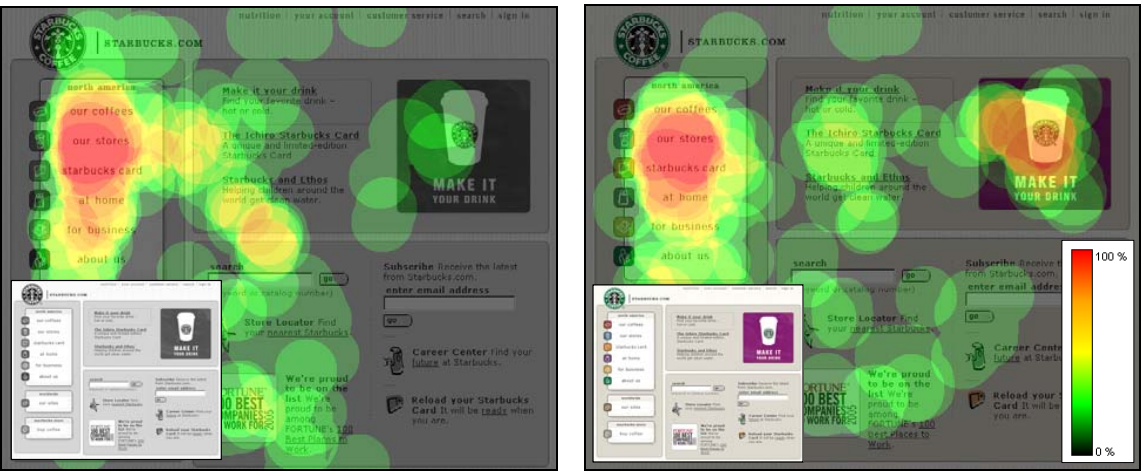
\includegraphics[width=\linewidth]{starbucks_bojko.png}
    \caption{Mapas de calor da busca pelo localizador de lojas na página da Starbucks. À esquerda, usuários ($n=13$) viram uma versão em preto e branco da página; à direita ($n=12$), a versão colorida. Cores mais quentes indicam maior porcentagem de usuários fixando o olhar na área. Fonte: \textcite{bojko2005eye}.}
    \Description{Dois mapas de calor sobre a página inicial da Starbucks.}
    \label{fig:starbucks_bojko}
\end{figure}

\textcite{pretorius2010} compararam usuários experientes e inexperientes em testes de usabilidade e mostraram que o rastreamento ocular revela problemas que não aparecem nos métodos tradicionais. \textcite{modi2022realtime} estudaram o olhar em uma rede social usando apenas uma câmera: o rosto é detectado, as regiões dos olhos são recortadas e uma CNN classifica a direção do olhar, permitindo gerar mapas de calor. O WebGazer \cite{papoutsaki2016webgazer} estima o olhar no próprio navegador, recalibrando-se continuamente a partir dos cliques do usuário. Entre as abordagens baseadas em aparência, \textcite{krafka2016eye} treinaram uma CNN com dados coletados de mais de 1.400 pessoas em celulares e \emph{tablets}, \textcite{zhang18_etra} mostraram a importância de normalizar a imagem do olho em relação à pose da cabeça, \textcite{Park2018ETRA} propuseram localizar pontos do olho com redes neurais para estimar o olhar em condições não controladas, e \textcite{Park2020ECCV} estimam o olhar a partir de vídeo de ponta a ponta. Por fim, \textcite{fuhl2020} utilizaram redes totalmente convolucionais para segmentar, gerar e reconstruir dados oculares brutos.

Este trabalho se diferencia por focar em um \emph{pipeline} completo, simples e aberto, que vai da imagem da webcam até as métricas de UX, e por reportar a qualidade dos dados com as métricas padronizadas de \textcite{holmqvist2012quality}, o que muitas vezes falta em protótipos com webcam.

%% ===========================================================================
\section{Materiais e Métodos}\label{sec:metodos}
%% ===========================================================================

\subsection{Visão geral}

O protótipo foi desenvolvido em duas etapas. Uma primeira versão, exploratória, usou HOG e o modelo de 68 pontos da dlib. As limitações observadas motivaram uma segunda versão, baseada no MediaPipe, que constitui o \emph{pipeline} avaliado neste trabalho (Figura~\ref{fig:pipeline}). O código está disponível em \url{https://github.com/brunoribas68/eyetracking}.

\begin{figure*}[t]
\centering
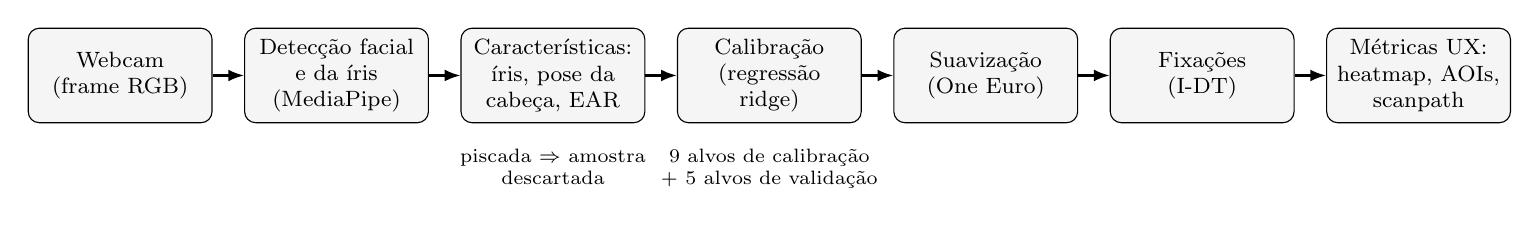
\begin{tikzpicture}[
  node distance=4mm,
  box/.style={draw, rounded corners, align=center, font=\footnotesize, minimum height=12mm, text width=21mm, fill=gray!8},
  arr/.style={-{Latex[length=2mm]}, thick}]
\node[box] (cam) {Webcam\\(frame RGB)};
\node[box, right=of cam] (det) {Detecção facial\\e da íris\\(MediaPipe)};
\node[box, right=of det] (feat) {Características:\\íris, pose da\\cabeça, EAR};
\node[box, right=of feat] (cal) {Calibração\\(regressão\\ridge)};
\node[box, right=of cal] (filt) {Suavização\\(One Euro)};
\node[box, right=of filt] (idt) {Fixações\\(I-DT)};
\node[box, right=of idt] (ux) {Métricas UX:\\heatmap, AOIs,\\scanpath};
\foreach \a/\b in {cam/det, det/feat, feat/cal, cal/filt, filt/idt, idt/ux} \draw[arr] (\a) -- (\b);
\node[font=\scriptsize, below=2mm of cal, text width=40mm, align=center] {9 alvos de calibração\\+ 5 alvos de validação};
\node[font=\scriptsize, below=2mm of feat, text width=26mm, align=center] {piscada $\Rightarrow$ amostra\\descartada};
\end{tikzpicture}
\caption{\emph{Pipeline} do protótipo: da imagem da webcam às métricas de experiência do usuário.}
\Description{Diagrama de blocos com sete etapas em sequência.}
\label{fig:pipeline}
\end{figure*}

\subsection{Protótipo inicial: HOG e 68 pontos faciais}

Na primeira versão, o rosto era detectado em tempo real com o detector HOG da dlib e, em seguida, os 68 pontos faciais eram estimados pelo modelo de árvores de regressão de \textcite{Kazemi2014}. A partir dos pontos que contornam cada olho, a região ocular era recortada (Figura~\ref{fig:hog_experimento}). Para localizar a pupila, a imagem era binarizada com um limiar ajustado manualmente, de modo que restassem apenas as regiões dos olhos (Figura~\ref{fig:apenas_olhos}), e o centro de cada região era marcado (Figura~\ref{fig:olhos_rastreados}).

\begin{figure}[t]
    \centering
    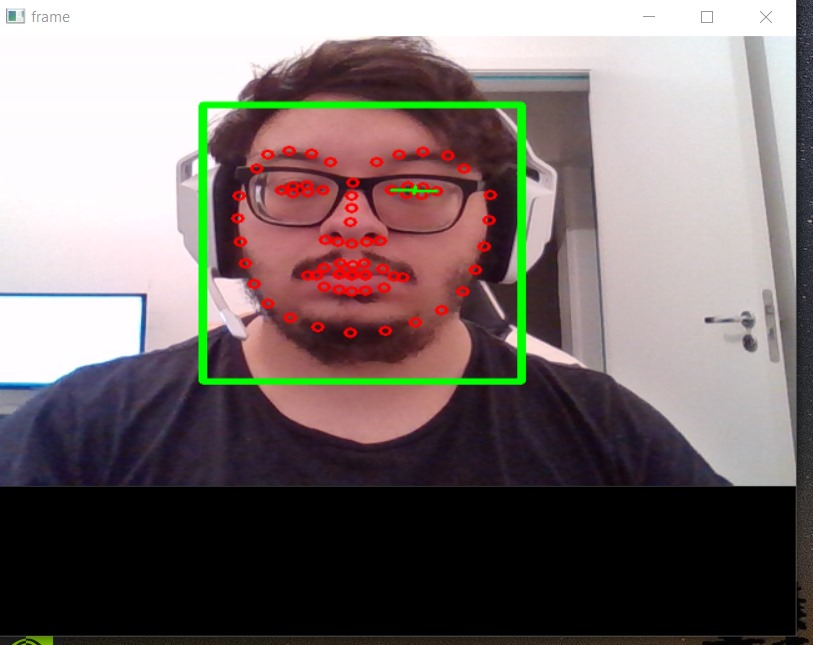
\includegraphics[width=\linewidth]{hog.jpg}
    \caption{Protótipo inicial. O quadrado verde indica o rosto detectado pelo HOG, os pontos vermelhos são os 68 pontos faciais e o traço verde marca o olho direito.}
    \Description{Rosto com os 68 pontos faciais marcados.}
    \label{fig:hog_experimento}
\end{figure}

\begin{figure}[t]
    \centering
    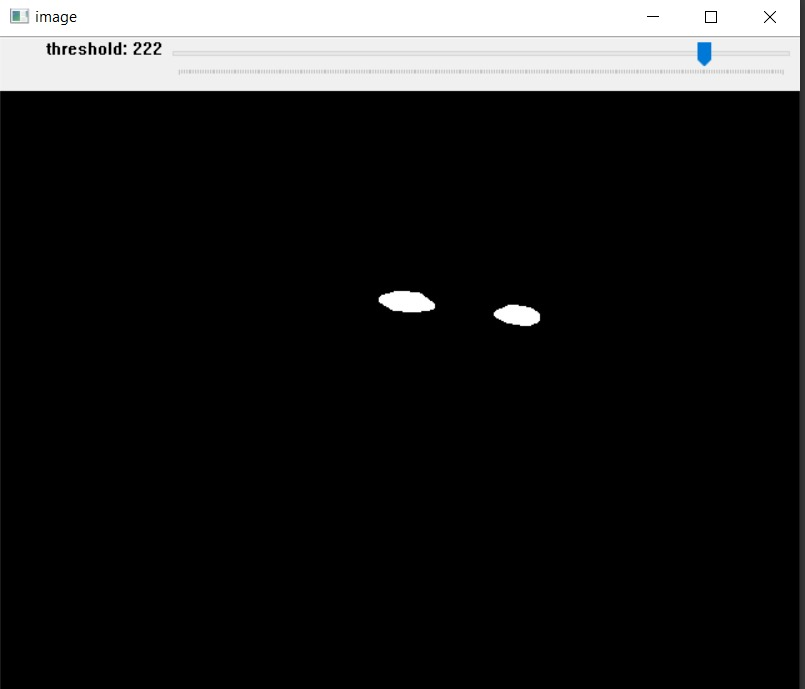
\includegraphics[width=\linewidth]{apenas_olhos.jpg}
    \caption{Binarização com limiar manual (222): apenas as regiões dos olhos permanecem.}
    \Description{Imagem binarizada com duas manchas brancas na posição dos olhos.}
    \label{fig:apenas_olhos}
\end{figure}

\begin{figure}[t]
    \centering
    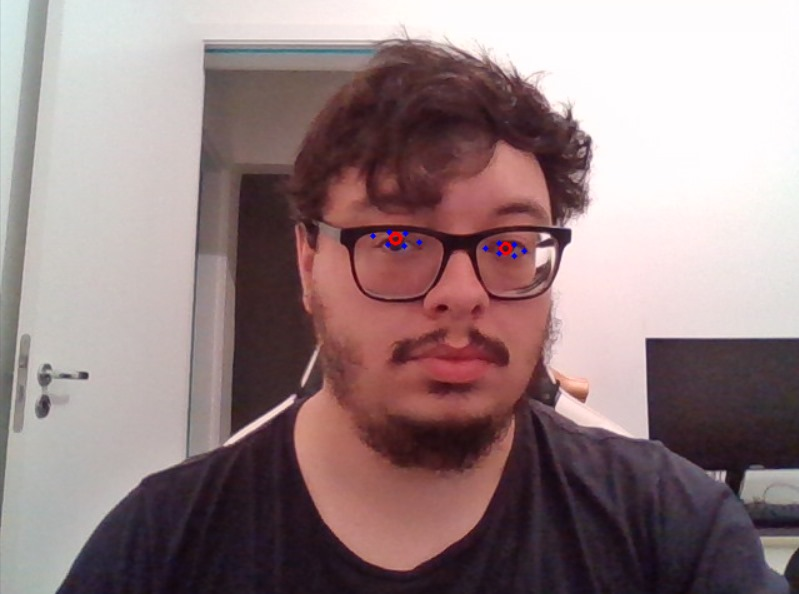
\includegraphics[width=\linewidth]{olhos_rastreados.jpg}
    \caption{Centros dos olhos marcados em vermelho sobre a imagem da webcam.}
    \Description{Rosto com os centros dos olhos marcados.}
    \label{fig:olhos_rastreados}
\end{figure}

Essa versão confirmou que é possível localizar os olhos em tempo real com uma webcam, mas revelou três limitações: (i) os 68 pontos contornam as pálpebras, mas não localizam a íris, de modo que a pupila dependia da binarização; (ii) o limiar de binarização precisava ser reajustado a cada mudança de iluminação e era afetado pelos reflexos das lentes de óculos; e (iii) não havia calibração, portanto o sistema localizava o olho, mas não o ponto observado na tela. A segunda versão foi construída para superar esses pontos.

\subsection{Pipeline final}

\subsubsection{Detecção e extração de características}
Cada \emph{frame} da webcam é processado pelo MediaPipe Face Mesh com o refinamento da íris \cite{kartynnik2019, ablavatski2020}. Para cada olho, sejam $\mathbf{c}$ o centro da íris (média dos seus cinco pontos), $\mathbf{m}$ o ponto médio entre os cantos interno e externo e $w$ a distância entre esses cantos. A posição normalizada da íris é
\begin{equation}
  e_x = \frac{c_x - m_x}{w}, \qquad e_y = \frac{c_y - m_y}{w},
\end{equation}
calculada como média dos dois olhos. A divisão por $w$ torna a medida independente da distância até a câmera. Para compensar parcialmente o movimento da cabeça, calcula-se também a posição da ponta do nariz $\mathbf{n}$ em relação ao ponto médio $\mathbf{o}$ entre os cantos externos dos olhos, normalizada pela distância interocular $d$: $(h_x, h_y) = (\mathbf{n} - \mathbf{o})/d$. O vetor de características de cada amostra é $\mathbf{z} = (e_x, e_y, h_x, h_y)$.

Piscadas são detectadas pela razão de aspecto do olho (\emph{eye aspect ratio}, EAR) \cite{soukupova2016}, aqui simplificada para a razão entre a abertura vertical e a largura do olho, $\mathrm{EAR} = \lVert \mathbf{p}_{sup} - \mathbf{p}_{inf} \rVert / w$. Como a EAR natural varia entre pessoas, o limiar é calibrado individualmente em uma pré-checagem de alguns segundos: o participante primeiro mantém os olhos abertos e depois pisca naturalmente, e o limiar é posicionado entre a mediana da EAR com olhos abertos e o percentil 5 da fase de piscadas. Amostras com piscada, ou em que o rosto não é detectado, são marcadas como perdidas. Como alternativa, o sistema pode usar o detector de Viola--Jones \cite{viola2001}, que não depende de redes neurais, mas não detecta piscadas.

\subsubsection{Calibração por regressão}
A calibração exibe, em tela cheia e em ordem aleatória, nove alvos em uma grade de $3\times3$ (a 10\%, 50\% e 90\% da largura e da altura). Cada alvo permanece por 2~s, e as amostras dos primeiros 0{,}7~s são descartadas para dar tempo ao olhar de se estabilizar. Em cada alvo, amostras atípicas são removidas por um critério robusto (mais de três desvios absolutos medianos da mediana). As características são padronizadas e o mapeamento para a tela $\hat{\mathbf{s}} = \mathbf{W}^\top \phi(\mathbf{z})$ é ajustado por regressão \emph{ridge}:
\begin{equation}
  \min_{\mathbf{W}} \sum_i \lVert \mathbf{s}_i - \mathbf{W}^\top \phi(\mathbf{z}_i) \rVert^2 + \lambda \lVert \mathbf{W}' \rVert^2,
\end{equation}
em que $\mathbf{s}_i$ é a posição do alvo, $\mathbf{W}'$ exclui o intercepto e $\lambda = 10^{-2}$. Foram avaliadas duas expansões: a linear, $\phi(\mathbf{z}) = (1, e_x, e_y, h_x, h_y)$, e a polinomial de segunda ordem, $\phi(\mathbf{z}) = (1, e_x, e_y, e_x e_y, e_x^2, e_y^2, h_x, h_y)$.

\subsubsection{Suavização e detecção de fixações}
As estimativas são suavizadas pelo filtro One Euro \cite{casiez2012}, um passa-baixas cuja frequência de corte aumenta com a velocidade do sinal: ele reduz o tremor quando o olhar está parado e introduz pouco atraso nas sacadas. O filtro é reiniciado após lacunas maiores que 200~ms. As fixações são identificadas pelo algoritmo I-DT \cite{salvucci2000identifying}, que agrupa amostras consecutivas cuja dispersão $D = (\max x - \min x) + (\max y - \min y)$ não excede um limiar. Foram usados dispersão máxima de 120~px, duração mínima de 100~ms e lacuna máxima de 100~ms dentro de uma fixação. \pendente{Justifique o limiar de 120 px em graus, com base na acurácia medida: ele deve ser maior que o ruído do sistema, senão uma única fixação é fragmentada em várias.}

\subsubsection{Validação e métricas de qualidade}
Após a calibração, cinco alvos \emph{novos} (quatro na grade de 30\% e 70\% e um no centro), que não participam do ajuste do modelo, são exibidos com o mesmo procedimento. Para cada alvo $\mathbf{t}$ com estimativas $\mathbf{p}_1, \dots, \mathbf{p}_n$, calculam-se \cite{holmqvist2012quality} a acurácia $\lVert \bar{\mathbf{p}} - \mathbf{t} \rVert$, a precisão RMS entre amostras sucessivas,
\begin{equation}
  \theta_{\mathrm{RMS}} = \sqrt{\frac{1}{n-1}\sum_{i=1}^{n-1} \lVert \mathbf{p}_{i+1} - \mathbf{p}_i \rVert^2},
\end{equation}
e a proporção de amostras perdidas. Os valores em pixels são convertidos para graus de ângulo visual a partir da largura física da tela $L$ (em cm), da sua resolução horizontal $R$ e da distância $D_o$ entre o olho e a tela:
\begin{equation}
  \text{px}/^\circ = \frac{R}{L} \cdot 2 D_o \tan(0{,}5^\circ).
\end{equation}
A validação é calculada com as estimativas brutas, sem suavização, para não mascarar a precisão real do sistema.

\subsection{Protocolo experimental}

\pendente{Preencher após realizar o experimento. Sugestão: 5 a 10 participantes já tornam o trabalho defensável.}

\textbf{Participantes.} Participaram \pendente{N} voluntários (\pendente{idade média, quantos usam óculos}). Nenhum vídeo é armazenado: o sistema grava apenas as características numéricas extraídas, o que reduz riscos à privacidade dos participantes. \pendente{Mencione o termo de consentimento, se houver.}

\textbf{Equipamento.} \pendente{Modelo do notebook ou computador, webcam e resolução da câmera, monitor (polegadas, resolução e largura física), distância aproximada de 60~cm, condições de iluminação.}

\textbf{Estímulo e tarefa.} \pendente{Sugestão que conversa com a Figura 1: um print da página inicial de um site com a tarefa ``encontre onde localizar uma loja'', exibido por 30~s. Defina as AOIs (menu, banner, busca, localizador etc.).}

\textbf{Procedimento.} Cada sessão segue a ordem: pré-checagem de detecção e piscada (6~s), calibração (9 alvos), validação (5 alvos) e exibição do estímulo com a tarefa. A sessão completa leva cerca de \pendente{2} minutos.

\textbf{Análise.} Para cada participante são calculadas as métricas de qualidade da validação e da gravação. Os modelos de calibração (linear e polinomial, com e sem as características da cabeça) são comparados \emph{offline}: cada modelo é treinado apenas com as amostras dos alvos de calibração e avaliado nos alvos de validação. Por fim, as fixações de todos os participantes são agregadas em um mapa de calor, e calculam-se, por AOI, o TTFF, o número de fixações, o tempo de permanência e o número de visitas.

\subsection{Tecnologias utilizadas}
O sistema foi implementado em Python, com OpenCV\footnote{\url{https://opencv.org/}} \cite{opencv} para captura e processamento de imagens, NumPy\footnote{\url{https://numpy.org/}} \cite{numpy} para a regressão e o processamento numérico, e MediaPipe\footnote{\url{https://ai.google.dev/edge/mediapipe}} \cite{lugaresi2019mediapipe} para o Face Mesh. O protótipo inicial usou a dlib\footnote{\url{http://dlib.net/}} \cite{King2009}. O repositório inclui testes automatizados, entre eles uma simulação completa da sessão com câmera e rosto sintéticos, usada para verificar o \emph{pipeline} antes dos experimentos com pessoas.

%% ===========================================================================
\section{Resultados e Discussão}\label{sec:resultados}
%% ===========================================================================

\pendente{Os valores desta seção saem diretamente dos arquivos gerados por analyze\_session.py (summary.csv, model\_comparison.csv, aoi\_metrics.csv).}

\subsection{Qualidade dos dados}

A Tabela~\ref{tab:qualidade} resume a qualidade dos dados de cada participante.

\begin{table}[t]
\caption{Qualidade dos dados por participante (modelo polinomial com pose da cabeça). Acurácia e precisão medidas nos alvos de validação.}
\label{tab:qualidade}
\begin{tabular}{lcccc}
\toprule
Part. & Acurácia ($^\circ$) & Precisão ($^\circ$) & Perda val. (\%) & Perda grav. (\%) \\
\midrule
P01 & \pendente{--} & \pendente{--} & \pendente{--} & \pendente{--} \\
P02 & \pendente{--} & \pendente{--} & \pendente{--} & \pendente{--} \\
\dots & & & & \\
\midrule
Média (DP) & \pendente{--} & \pendente{--} & \pendente{--} & \pendente{--} \\
\bottomrule
\end{tabular}
\end{table}

\pendente{Comente: a acurácia média é compatível com o que a literatura relata para webcam? Algum participante destoou (óculos, iluminação)? Lembre que rastreadores infravermelhos ficam abaixo de 1$^\circ$. Compare com os números reportados nos trabalhos relacionados, conferindo-os nos artigos originais.}

\subsection{Comparação dos modelos de calibração}

\begin{table}[t]
\caption{Acurácia média na validação (graus) por modelo de calibração, treinado apenas com os alvos de calibração.}
\label{tab:modelos}
\begin{tabular}{lcc}
\toprule
Modelo & Com pose da cabeça & Sem pose da cabeça \\
\midrule
Linear & \pendente{--} & \pendente{--} \\
Polinomial (2ª ordem) & \pendente{--} & \pendente{--} \\
\bottomrule
\end{tabular}
\end{table}

\pendente{Discuta a Tabela~\ref{tab:modelos}. O modelo polinomial tem mais parâmetros: ele generaliza melhor para os alvos de validação ou sobreajusta os 9 pontos? A pose da cabeça ajuda? Qualquer resultado é válido e interessante, desde que seja o resultado real.}

\subsection{Aplicação em experiência do usuário}

\begin{figure}[t]
  \centering
  \IfFileExists{group_heatmap.png}{%
    \includegraphics[width=\linewidth]{group_heatmap.png}}{%
    \fbox{\parbox[c][4cm][c]{0.9\linewidth}{\centering\pendente{Inserir group\_heatmap.png gerado pelo analyze\_session.py}}}}
  \caption{Mapa de calor agregado das fixações dos \pendente{N} participantes durante a tarefa \pendente{descrever a tarefa}.}
  \Description{Mapa de calor sobre a página usada como estímulo.}
  \label{fig:heatmap}
\end{figure}

\begin{table}[t]
\caption{Métricas por área de interesse (média entre participantes).}
\label{tab:aoi}
\begin{tabular}{lcccc}
\toprule
AOI & Encontraram (\%) & TTFF (s) & Fixações & Permanência (s) \\
\midrule
\pendente{menu} & \pendente{--} & \pendente{--} & \pendente{--} & \pendente{--} \\
\pendente{busca} & \pendente{--} & \pendente{--} & \pendente{--} & \pendente{--} \\
\bottomrule
\end{tabular}
\end{table}

\pendente{Interprete a Figura~\ref{fig:heatmap} e a Tabela~\ref{tab:aoi} como um pesquisador de UX faria: o elemento-alvo foi encontrado? Em quanto tempo? Que região atraiu atenção sem ser útil para a tarefa? Relacione com Norman (visibilidade, affordances) e com a Figura~\ref{fig:starbucks_bojko}.}

\subsection{Limitações e ameaças à validade}

A pose da cabeça é estimada de forma aproximada, a partir de pontos 2D; movimentos amplos após a calibração degradam o mapeamento, o que exigiria recalibração ou apoio de queixo. Óculos com reflexo, pouca iluminação e contraluz aumentam a perda de dados. A taxa de amostragem é limitada pela webcam (tipicamente 30~Hz), insuficiente para medir sacadas com precisão, de modo que o trabalho se restringe a métricas baseadas em fixações. Por fim, a amostra de participantes é pequena e não representativa, e os resultados devem ser lidos como uma avaliação de viabilidade, não como uma validação definitiva. \pendente{Acrescente limitações observadas na prática.}

%% ===========================================================================
\section{Considerações Finais}\label{sec:conclusao}
%% ===========================================================================

Este trabalho desenvolveu um protótipo de rastreamento ocular baseado apenas em uma webcam e em técnicas de Inteligência Artificial, com o objetivo de obter dados úteis para avaliar a experiência do usuário. A evolução de um primeiro protótipo, baseado em HOG e em árvores de regressão, para um \emph{pipeline} com uma CNN de detecção da íris, calibração por regressão regularizada, filtragem adaptativa e detecção de fixações permitiu passar da simples localização dos olhos para a estimativa do ponto observado na tela e para métricas de UX.

\pendente{Retome cada objetivo específico e diga se foi atingido, com os números principais: acurácia, precisão, perda de dados, melhor modelo de calibração e o principal achado de UX.}

\pendente{Conclusão honesta sobre a viabilidade. Por exemplo: a acurácia obtida permite identificar quais regiões de uma página recebem atenção, desde que as AOIs sejam grandes em relação ao erro, mas não substitui um rastreador dedicado em análises finas, como a leitura.}

Como trabalhos futuros, destacam-se: substituir o mapeamento por características por modelos baseados em aparência com normalização da pose da cabeça \cite{zhang18_etra, Park2018ETRA}; recalibrar o modelo continuamente a partir das interações do usuário, como no WebGazer \cite{papoutsaki2016webgazer}; avaliar o uso de apenas um olho quando ele for mais confiável \cite{hooge2019}; e portar o sistema para o navegador, permitindo testes de UX remotos com um número maior de participantes.

\printbibliography

\end{document}
